% 
% exemplo genérico de uso da classe iiufrgs.cls
% $Id: iiufrgs.tex,v 1.1.1.1 2005/01/18 23:54:42 avila Exp $
%
% This is an example file and is hereby explicitly put in the
% public domain.
%
\documentclass[tuberlin,cic,tc,openright,english,noabntcite]{iiufrgs}
% Para usar o modelo, deve-se informar o programa e o tipo de documento.
% Programas :
% * cic       -- Graduação em Ciência da Computação
% * ecp       -- Graduação em Ciência da Computação
% * ppgc      -- Programa de Pós Graduação em Computação
% * pgmigro   -- Programa de Pós Graduação em Microeletrônica
% * tuberlin  -- Bachelorarbeit entregue na TU Berlin
%
% Tipos de Documento:
% * tc                -- Trabalhos de Conclusão (apenas cic e ecp)
% * diss ou mestrado  -- Dissertações de Mestrado (ppgc e pgmicro)
% * tese ou doutorado -- Teses de Doutorado (ppgc e pgmicro)
% * ti                -- Trabalho Individual (ppgc e pgmicro)
%
% Outras Opções:
% * english    -- para textos em inglês
% * openright  -- Força início de capítulos em páginas ímpares (padrão da
% biblioteca)
% * oneside    -- Desliga frente-e-verso
% * nominatalocal -- Lê os dados da nominata do arquivo nominatalocal.def


% Use unicode
\usepackage[utf8]{inputenc}   % pacote para acentuação

% Necessário para incluir figuras
\usepackage{graphicx}         % pacote para importar figuras
\graphicspath{ {img/} }

\usepackage{times}            % pacote para usar fonte Adobe Times
% \usepackage{palatino}
% \usepackage{mathptmx}       % p/ usar fonte Adobe Times nas fórmulas

%\usepackage[alf,abnt-emphasize=bf]{abntex2cite}	% pacote para usar citações abnt
\usepackage[round]{natbib}

\usepackage{subcaption} %Support for sub figures

%
% Informações gerais
%
\title{Towards Synchronizing Relations Between Artifacts in the Java Technological Space}

\author{Bombardelli da Silva}{William}
% alguns documentos podem ter varios autores:
% \author{Flaumann}{Frida Gutenberg}
% \author{Flaumann}{Klaus Gutenberg}

% orientador e co-orientador são opcionais (não diga isso pra eles :))
\advisor[Prof.~Dr.]{}{}
%\coadvisor[Prof.~Dr.]{Knuth}{Donald Ervin}

% a data deve ser a da defesa; se nao especificada, são gerados
% mes e ano correntes
% \date{maio}{2001}

% o local de realização do trabalho pode ser especificado (ex. para TCs)
% com o comando \location:
\location{Berlin}{Germany}

% itens individuais da nominata podem ser redefinidos com os comandos
% abaixo:
% \renewcommand{\nominataReit}{Prof\textsuperscript{a}.~Wrana Maria Panizzi}
% \renewcommand{\nominataReitname}{Reitora}
% \renewcommand{\nominataPRE}{Prof.~Jos{\'e} Carlos Ferraz Hennemann}
% \renewcommand{\nominataPREname}{Pr{\'o}-Reitor de Ensino}
% \renewcommand{\nominataPRAPG}{Prof\textsuperscript{a}.~Joc{\'e}lia Grazia}
% \renewcommand{\nominataPRAPGname}{Pr{\'o}-Reitora Adjunta de P{\'o}s-Gradua{\c{c}}{\~a}o}
% \renewcommand{\nominataDir}{Prof.~Philippe Olivier Alexandre Navaux}
% \renewcommand{\nominataDirname}{Diretor do Instituto de Inform{\'a}tica}
% \renewcommand{\nominataCoord}{Prof.~Carlos Alberto Heuser}
% \renewcommand{\nominataCoordname}{Coordenador do PPGC}
% \renewcommand{\nominataBibchefe}{Beatriz Regina Bastos Haro}
% \renewcommand{\nominataBibchefename}{Bibliotec{\'a}ria-chefe do Instituto de Inform{\'a}tica}
% \renewcommand{\nominataChefeINA}{Prof.~Jos{\'e} Valdeni de Lima}
% \renewcommand{\nominataChefeINAname}{Chefe do \deptINA}
% \renewcommand{\nominataChefeINT}{Prof.~Leila Ribeiro}
% \renewcommand{\nominataChefeINTname}{Chefe do \deptINT}

% A seguir são apresentados comandos específicos para alguns
% tipos de documentos.

% Relatório de Pesquisa [rp]:
% \rp{123}             % numero do rp
% \financ{CNPq, CAPES} % orgaos financiadores

% Trabalho Individual [ti]:
% \ti{123}     % numero do TI
% \ti[II]{456} % no caso de ser o segundo TI

% Monografias de Especialização [espec]:
% \espec{Redes e Sistemas Distribuídos}      % nome do curso
% \coord[Profa.~Dra.]{Weber}{Taisy da Silva} % coordenador do curso
% \dept{INA}                                 % departamento relacionado

%
% palavras-chave
% iniciar todas com letras minúsculas, exceto no caso de abreviaturas
%
\keyword{formatação eletrônica de documentos}
\keyword{\LaTeX}
\keyword{ABNT}
\keyword{UFRGS}

%\settowidth{\seclen}{1.10~}

%
% inicio do documento
%
\begin{document}

% folha de rosto
% às vezes é necessário redefinir algum comando logo antes de produzir
% a folha de rosto:
% \renewcommand{\coordname}{Coordenadora do Curso}
\maketitle

% dedicatoria
% \clearpage
% \begin{flushright}
%     \mbox{}\vfill
%     {\sffamily\itshape
%       ``If I have seen farther than others,\\
%       it is because I stood on the shoulders of giants.''\\}
%     --- \textsc{Sir~Isaac Newton}
% \end{flushright}

% agradecimentos
%\chapter*{Agradecimentos}
%Agradeço ao \LaTeX\ por não ter vírus de macro\ldots



% resumo na língua do documento
\begin{abstract}
    Este documento é um exemplo de como formatar documentos para o
    Instituto de Informática da UFRGS usando as classes \LaTeX\
    disponibilizadas pelo UTUG\@. Ao mesmo tempo, pode servir de consulta
    para comandos mais genéricos. \emph{O texto do resumo não deve
      conter mais do que 500 palavras.}
\end{abstract}

% resumo na outra língua
% como parametros devem ser passados o titulo e as palavras-chave
% na outra língua, separadas por vírgulas
\begin{englishabstract}{Using \LaTeX\ to Prepare Documents at II/UFRGS}{Electronic document preparation. \LaTeX. ABNT. UFRGS}
    This document is an example on how to prepare documents at II/UFRGS
    using the \LaTeX\ classes provided by the UTUG\@. At the same time, it
    may serve as a guide for general-purpose commands. \emph{The text in
      the abstract should not contain more than 500~words.}
\end{englishabstract}

% lista de figuras
\listoffigures

% lista de tabelas
\listoftables

% lista de abreviaturas e siglas
% o parametro deve ser a abreviatura mais longa
\begin{listofabbrv}{SPMD}
    \item[SMP] Symmetric Multi-Processor
    \item[NUMA] Non-Uniform Memory Access
    \item[SIMD] Single Instruction Multiple Data
    \item[SPMD] Single Program Multiple Data
    \item[ABNT] Associação Brasileira de Normas Técnicas
\end{listofabbrv}

% idem para a lista de símbolos
% \begin{listofsymbols}{$\alpha\beta\pi\omega$}
%     \item[$\sum{\frac{a}{b}}$] Somatório do produtório
%     \item[$\alpha\beta\pi\omega$] Fator de inconstância do resultado
% \end{listofsymbols}

% sumario
\tableofcontents

% aqui comeca o texto propriamente dito

% introducao
\chapter{Introduction}
%TODO: Quotes
The techniques for software development has changed in the course of time since the rise of general-purpose programmable computers and specially in the second half of the 20th century with the rise of digital computers [QUOTE computing history]. In the beginning of digital computer programming machine code was used to describe algorithms, but as complexity and size of such algorithms got bigger this technique soon became impracticable and evoked the need for a more sophisticated way of programming these digital computers. The assembly languages (also known as low-level programming languages) came to solve this problem, but clearly the complexity kept increasing as well as the need for new techniques and technologies for software programming [QUOTE languages history]. The popularization of computing, and the increasing application of computers in the practice urged the creation of high-level programming languages (e.g. Cobol, Fortran), which kept evolving mainly in regard to the needs of the software market [QUOTE languages history]. More sophisticated languages (e.g. C, Pascal) and new paradigms (e.g. modular and object-oriented programming) also arose in the late 20th century. But the evolution of software development does not seem to stop, evidenced by the lately increasing research on new software engineering techniques such as the Model-driven Engineering.

The newest characteristics of the information system market, like the constant evolution of the software systems, the interoperability between them and the big number of developers working in a common software artifact has required the use of software models; and the research on how to apply systematically and correctly such models in the development processes, what is called Model-driven Engineering or Model-driven Software Development [QUOTE MDE]. This Bachelor thesis aims therefore to explore one specific realm of Model-driven Engineering research, namely the synchronization problem between models (or artifacts) in the Java technological space. The goal here is to pick commonly used meta-models in Java systems, describe them and identify their relations, so that they can be synchronized.

%TODO: Remainder
TALK ABOUT THE REMAINDER OF THE DOCUMENT.

\section{Background}
%TODO artifacts = models ?
According to \citet[p. 21]{czarnecki2006feature}: "\textit{Models are system abstractions that allow developers and other stakeholders to effectively address concerns, such as answering a question about the system or effecting a change}”. By defining a model as a system abstraction, it becomes clear, that a software system might have several models abstracted from it, each one representing certain aspects of the whole system. These models also have relations between them, in the sense that they all are supposed to describe the actual system consistently by not presenting logical contradictions. Here examples of models are \emph{UML class diagram}, \emph{Use Cases}, or even the source-code itself. The term model and artifacts will be used interchangeably throughout this document (?).
%TODO: QUOTE
%TODO: First person plural is ok?
The constant evolving nature of current large-scale software systems causes its models to be constantly changed [QUOTE]. But in order to maintain this whole network of interconnected models consistent the changes have to be forwarded through the network, i.e. all models have to be synchronized. Suppose one have a \emph{UML Class Diagram}, a series of \emph{UML Sequence Diagrams} and the source-code. If a method has its name changed in the class diagram, all occurrences of this method has to have its name updated in the sequence diagrams and in the source-code. It turns out though, that neither a model synchronization tool comprising the most common meta-models used nowadays in Java information systems is known by us nor have we found clearly defined relation definitions between them on the literature. 

\section{Objective}
The goal of this bachelor thesis is first to choose software meta-models commonly used in current Java object oriented software systems, writing down the meta-model definitions; second to define the relations between the chosen meta-models; and last, to showcase how these artifacts can be synchronized in some representative cases. We work therefore with the hypothesis, that such meta-models can be found and defined; that some relations between them can be written in some language; and that some of these relation can be synchronized using a tool or technique available in the current literature.

The end of this document shall present all the written definitions as well as the results of the synchronization of representative examples useful in the practice. Furthermore, the report of this thesis recording the difficulties and experiences found during the work process and an analysis and discussion of future development and challenges of the realm is also a legacy.

\section{Motivation}
%TODO: us again
The lack of a functional model synchronization tool integrating a broad range of meta-models used currently in Java software engineering is the main motivation for this thesis. Although an expressive effort has been made by the academic community to create solutions for the problem of model synchronization, no study known by us presents an effective tool, that could be used extensively in practice. We believe though, that the contribution of this thesis can be useful for the creation of such a tool.
	
Another motivation for this thesis is the lack of relation definitions in current literature for extensively used meta-models in Java systems industry. Examples of these relations include relations between \emph{UML Class and Sequence Diagrams} and \emph{Java Code}, between \emph{Use Cases} and \emph{Requirements Diagrams}, between \emph{OCL contracts (used in design by contract methods)} and \emph{Unit Tests}, among others. It means, that the success of this thesis brings the contribution towards the definition of a network of interconnected meta-models useful to both research and industry community. Therefore the availability of such a network might finally allow the extensive use of Model-driven Engineering in practice $-$ helping bridging the gap between system abstractions and their concrete form $-$ and foster the further development of more sophisticated model synchronization methods.

%TODO: Quote
It is worth to note also, that the contribution of this thesis might help enhancing the quality of current software construction and therefore lessening the number of software problems and errors, what is an endemic problem nowadays [QUOTE], by fomenting the wide application of Model-Driven Software Development.

\section{Methodology}
In order to achieve the goals the following procedure is taken. In the first moment a collection of common meta-models used in the Java technological space are to be defined, this is done through an state-of-art research, once some meta-models have already been defined by other authors, plus the creation of our own versions of some meta-models, that are not available in the state-of-art. So for example, in this phase the choice of applied meta-models (i.e. \emph{UML Class Diagram} and \emph{Java Code}) will be done and their definitions will be written.

%TODO: Link def TGG
Later on, given the defined meta-models, the relations between them can be written. So for example, in this phase the inherent relation between the \emph{UML Class Diagram} meta-model and the \emph{Java Code} meta-model will be written. Analogously, the relations between \emph{Java Code}, \emph{JavaDoc}, \emph{UML Sequence Diagram} and other meta-models of the Java technological space are also to be defined. All of these relations are developed during the work of this thesis.

%TODO: Synchronization?
After having this network of meta-models ready, creating an actual network of concrete models of any software system is trivial, thus a showcase using a synchronization method from the current academic literature is applied to illustrate the synchronization between some representative meta-models.

%TODO: Scope / LIMITS

\chapter{Bibliographic Background}
Before describing the development of this thesis is important to review the academic state-of-art of model synchronization as well as to review some important definitions regarded to Model-driven Engineering.

\section{Important Definitions}
Below is a list of necessary basic concepts definition, that will be used throughout this document. Some of these definitions are rather narrower than they could be, but for the scope of this thesis they seem to be suitable.
%TODO: \emph in the citings

%TODO: QUOTE
\begin{description}
\item[Technological Space:] According to the definition from \citet[p. 1]{kurtev2002technological}: \emph{"A technological space is a working context with a set of associated concepts, body of knowledge, tools, required skills, and possibilities. It is often associated to a given user community with shared know-how, educational support, common literature and even workshop and conference meetings"}. By \emph{Java Techonological Space} is meant the set of commonly used models, practices, techniques and technologies in Java software development. For example, object-oriented development, unit tests, code documentation and the Java Virtual Machine are items of the \emph{Java Techonological Space}.

\item[System:] The term system is used interchangeably with the terms software, or program. And is intended to represent a software unit that abstracts a reality (or problem) and is abstracted by one or more models.

%TODO: Quote Exact page
%TODO: artifacts = models?
\item[Model:] The definition for software model used is given by [QUOTE SEIDEWITZ]: "A model is a set of statements about some system under study (SUS). Here, statement means some expression about the SUS that can be considered true or false". According to them, models can be used (1) to describe a system, in this case the model makes statements about the SUS, an example is an \emph{UML sequence diagram} employed to help understand the behavior of a Java system. But models can also be used (2) to specify a system, in this case it is used in the validation of the system, an example is a \emph{UML class diagram} employed as design specification of a Java system. Further examples of models, according to this definition, are a \emph{relational database diagram} of a database, the documentation of a system in \emph{Java Doc} or even a Java source-code. The term \emph{artifact} is used as a synonym for model. (?)

%TODO: Link model
%TODO: Quote page
\item[Modeling Language:] If, according to [LINK MODEL DEF], a model is a set of statements, one needs a way to express such statements. Therefore "A modeling language lets us express the statements in models of some class of SUS" [QUOTE SEIDEWITZ]. Examples of modeling languages are the \emph{UML}, the \emph{diagram notation for relational database diagram} or the Java language.

%TODO: Quote exact page
%TODO: Link
\item[Meta-model:] [QUOTE SEIDEWITZ] affirms: "A metamodel is a specification model for a class of SUS where each SUS in the class is itself a valid model expressed in a certain modeling language", that means, a meta-model is a model used to specify another model. Furthermore, "a metamodel makes statements about what can be expressed in the valid models of a certain modeling language" [QUOTE SEIDEWITZ]. In other words, a meta-model specifies what can be written using a certain modeling language. Thus, examples of meta-models are \emph{UML specification document} [QUOTE UML], the \emph{entity-relationship meta-model} [QUOTE ER PDF 54] or the Java meta-model (one example is to be found in [QUOTE JAMOPP]). Finally [QUOTE SEIDEWITZ] also claims: "Because a metamodel is a model, we express it in some modeling language". One example of a modeling language for meta-models is the \emph{EMF Ecore} [QUOTE].

%TODO: Links
%TODO: Quote MOF
\item[Meta-metamodel:] Analogously to the meta-model definition [LINK], "a meta-metamodel is a specification model of a class of SUS where each SUS is itself a valid meta-model expressed in a certain meta-modeling language". To put in other words, a meta-metamodel is a model used to specify another meta-model. Examples of meta-metamodels are the \emph{MOF}[QUOTE] or the \emph{XML} [QUOTE search too]. It is to note also, that such derivation can be done iteratively in the sense that a $meta^3-model$ definition is also possible, although it is not useful for the scope of this thesis. The figures [LINK 1 + 2] illustrate our understanding of the definitions above.

%TODO: Remove space in this spot
\begin{figure}[h]
    \caption{Depiction of the theoretical definitions of system, model, metamodel, meta-metamodel and modeling language. Like stated before, a system is abstracted by models, which themselves are abstracted by meta-models and so forth. A model used to specify (see the model definition) has a red line binding it and its SUS labeled with the identifier of the respective modeling language.}
    \begin{center}
        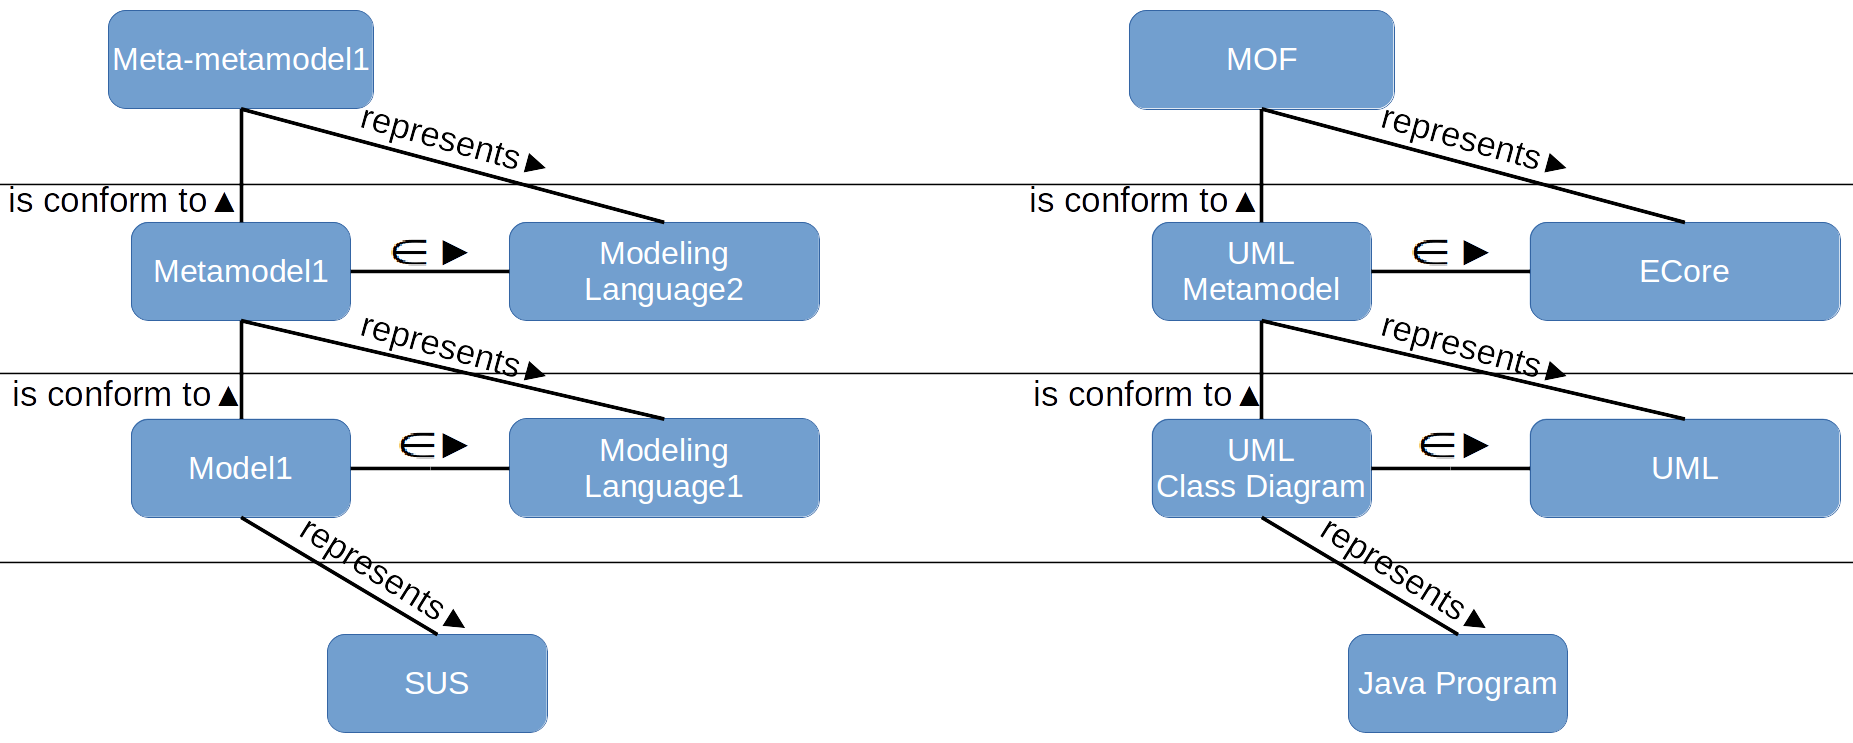
\includegraphics[width=25em]{model_scheme}
    \end{center}
    \label{fig:model_scheme}
    \legend{Source: The author}
\end{figure}
%TODO: Link
\begin{figure}[h]
    \caption{A more concrete and practical illustration of the definitions of system, model, metamodel, meta-metamodel and modeling language. This example shows a scenario very close to the implementation made in [LINK CHAPTER MODEl]}
    \begin{center}
        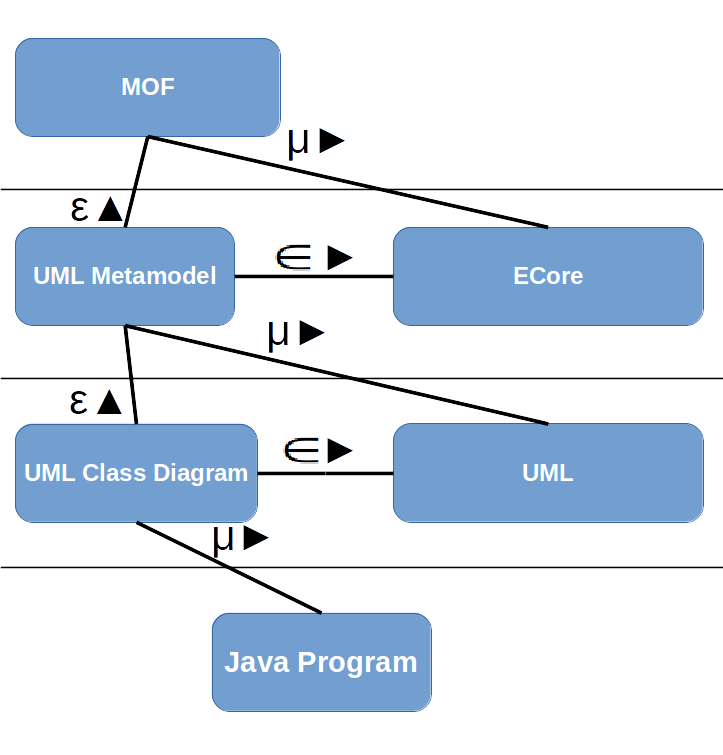
\includegraphics[width=25em]{model_scheme_practice}
    \end{center}
    \label{fig:model_scheme_practice}
    \legend{Source: The author}
\end{figure}
	
\item[Model Relation:] Model relation here is defined abstractly as every relationship or constraint possible to happen between one source model and one target model. For instance, the models \emph{UML class diagram} and Java code have a relation, because once a new class is created in the class diagram, the correspondent class has to be created in the Java code. Moreover, a \emph{UML class diagram} with contracts definitions (pre and post-conditions) have a relation to the \emph{JUnit model}, once that the formers have to be tested correspondingly in the latter.

%TODO: Note that? ok?
\item[Model Transformation:] Model transformation can be viewed as common data transformation – very common in computer science – with the specificity of dealing with models \cite{czarnecki2006feature}. More specifically, model transformation is defined here as a function $t : M \rightarrow N$, where $t(m) = n$ means that a target model $n \in N$ is created from a source model $m \in M$, $M$ and $N$ being respectively the set of all valid models of the meta-models $\Phi_M$ and $\Phi_N$. Practical example: Creation of Java code from \emph{UML class diagram}. Note that, model transformation is by nature deterministic, unidirectional and does not preserve the information of the target model (e.g. comments in the Java code).

%TODO: Note that? ok?
%TODO: LINK
\item[Model Synchronization:] The goal of model synchronization is to maintain all relations between the models of a system consistent/correct as updates are performed over them \cite{diskin2011model}. More specifically, model synchronization is defined here as a function $s : M x M x N x N \rightarrow M x N $, where $s(m_0,m_1,n_0,n_1) = (m_2,n_2)$ means that final synchronized models $m_2$ and $n_2$ are created from the initial synchronized models $m_0$ and $n_o$ and the modified non-synchronized models $m_1$ and $n_1$. Practical example: Modification of a method name in the \emph{UML class diagram} has to be forwarded to the Java code, without losing extra information of it (e.g. comments). Note that, model synchronization is deterministic, bidirectional and preserves the informations of the both models. The image [LINK] summarizes the ideas of model and model synchronization. Other terms for model synchronization used interchangeably throughout this document are iterative or information preserving bidirectional model transformation.

%TODO: LINK + QUOTE
\item[Network of Models:] A network of models of a system $S$ is an undirected graph $G = (V,E)$, whereas each vertex $v_i \in V$ represents a unique model $i$ abstracting $S$, and an edge $(v_i, v_j)$ exists if, and only if there is a relation defined between both models $i$ and $j$. In the figure [LINK] is an example of a network of models, illustrating the possible complexity of such network. More discussion is to find on [QUOTE 56].

\begin{figure}[h]
    \caption{An example of a network of models very similar to the one developed in this work.}
    \begin{center}
        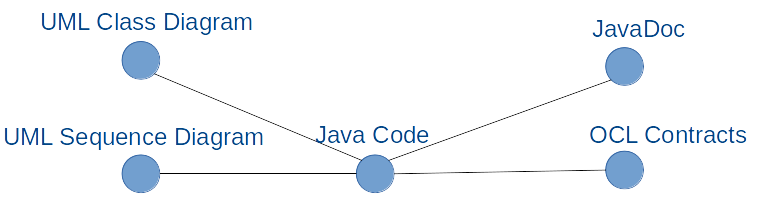
\includegraphics[width=25em]{network_example_01}   
    \end{center}
    \label{fig:network_example_01}
    \legend{Source: The Author}
\end{figure}

\item[Meta Object Facility:] "The Meta Object Facility (MOF) provides an open and platform-independent metadata management framework and associated set of metadata services to enable the development and interoperability of model and metadata driven systems" [QUOTE 31]. The MOF describes therefore the MOF modeling language, which is used to model the meta-metamodel utilized in this thesis. Essentially, it inherits much from the UML and deals with the ideas of classes, properties and associations, providing and extensible but simple fashion to define meta-models. The figure [LINK] shows the essential part of MOF.

\begin{figure}[h]
    \caption{Essential MOF definition, which handles basically classes, properties, operations, associations, and generalization.}
    \begin{center}
        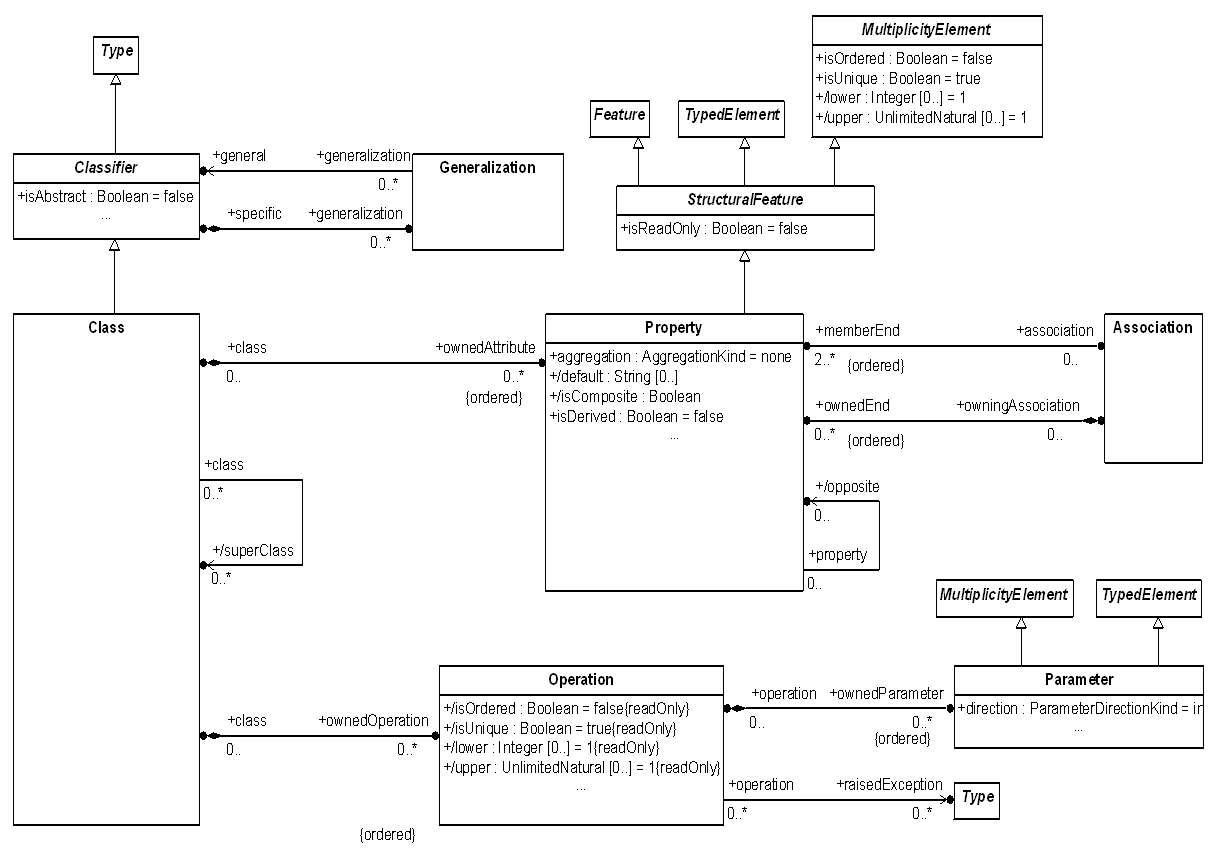
\includegraphics[width=35em]{emof_classes}   
    \end{center}
    \label{fig:emof_classes}
    \legend{Source: [QUOTE 31 pg. 27]}
\end{figure}

%TODO: Site +  link
\item[Ecore:] Ecore\footnote{SITE} is the meta-metamodel utilized in this thesis to describe all the applied meta-models (e.g the Java meta-model). Ecore is an initiative of the EMF Project\footnote{SITE} and aims to provide not only a meta-metamodel but a set of tools for criating meta-models, like an Eclipse plug-in generation feature, that enables the model developer to easily test and debug its meta-models. The Ecore meta-metamodel is at least similar to the essential MOF standard, and that is the reasons it is applied here. A proof of sich compliance is not know by us though. The figure [LINK] shows the essential part of Ecore.


%TODO: link +  data site
\begin{figure}[h]
    \caption{Ecore definition illustrating the use of classes, attributes, operations, references and super types, analougously to the figure [LINK EMOF FIG]}
    \begin{center}
        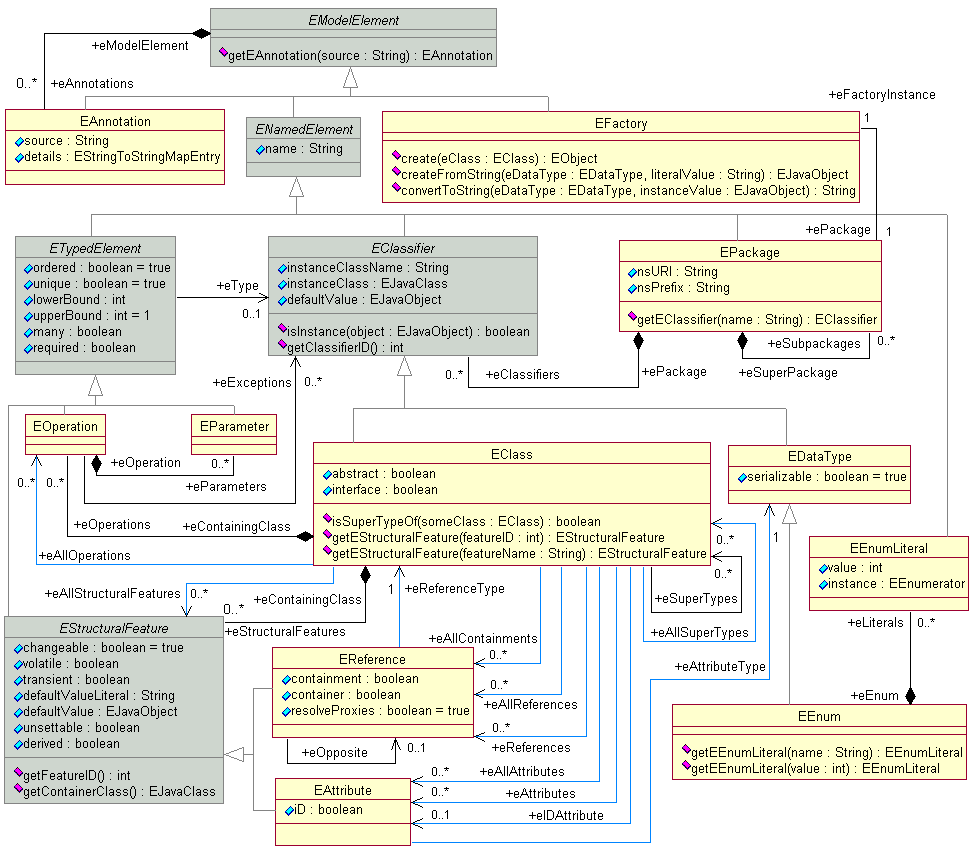
\includegraphics[width=35em]{ecore_relations}   
    \end{center}
    \label{fig:ecore_relations}
    \legend{Source: http://download.eclipse.org/modeling/emf/emf/javadoc/2.9.0/org/eclipse/emf/ecore/package-summary.html}
\end{figure}

%TODO: Link
%TODO: quote
\item[Triple Graph:] With the use of a triple graph a relation between a source model S and a target model T are abstracted into a triple $(G_s,G_c,G_t)$ – where $G_s$ is the graph representation of source model elements, $G_t$ is the graph representation of target model elements, and $G_c$ represents the correspondence between the two set of model elements – together with two mappings $s_g: G_c \rightarrow G_s$ and $t_g: G_c \rightarrow G_t$, which bind the three graphs [QUOTE HERMANN].

In this case, a modification in the triple graph $G = (G_s,G_c,G_t)$, that leads to a new triple graph $H = (H_s,H_c,H_t)$ consists in a triple graph morphism $m: G \rightarrow H$, with $m = (m_s,m_c,m_t)$. According to the figure [LINK].

%TODO: quote
\begin{figure}[h]
    \caption{The morphism $m: G \rightarrow H$ is a triple graph $m = (m_s,m_c,m_t)$.}
    \begin{center}
        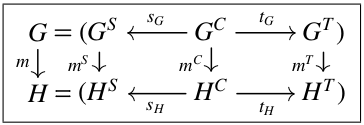
\includegraphics[width=20em]{tg_morphism}   
    \end{center}
    \label{fig:tg_morphism}
    \legend{Source: [Hermann 2011]}
\end{figure}

%TODO: quote
\item[Triple Rule:] A triple rule is a triple graph morphism $t_r = (s, c, t) : L \rightarrow R$, where $L$ and $R$ are called respectively the left-hand the right-hand sides \citep{ehrig2007information}.

\item[Triple Axiom:] A triple axiom is a triple rule $t_a = (s, c, t) : \emptyset \rightarrow R$. In order to apply such definitions in the practice, it is common to use attributed graphs and a easier to read diagram scheme depicted in the figure [LINK].

%TODO: Take figure from development
\begin{figure}[h]
    \caption{TRIPLE GRAPH, TRIPLE RULE, TRIPLE AXIOM, explain ++}
    \begin{center}
        %\includegraphics[width=20em]{}   
    \end{center}
    \label{fig:triple_rules}
    \legend{Source: The author}
\end{figure}

%TODO: Link
\item[Triple Graph Grammar:] A triple graph grammar $TGG = (t_a, T_rules) $ consists of a triple axiom $t_a$ and a set of triple rules $T_rules$ [QUOTE 44 PG 4]. While triple graphs are used as a description of the relations between two meta-models, TGG's describe the semantics of the transformation procedure, where triple rules correspond to operational rules of the formal semantic (see [LINK synchronization section]).

\begin{figure}[h]
    \caption{Illustration of the definitions model relation, transformation and synchronization as well as triple graph grammars (TGG). Relations between metamodels are coded by triple grammars; modifications in the models are coded by triple rules, which are then organized in a TGG. A TGG is interpreted as operational semantic definitions and executed according to the models. Again the concept of modeling language is pictured as red lines.}
    \begin{center}
        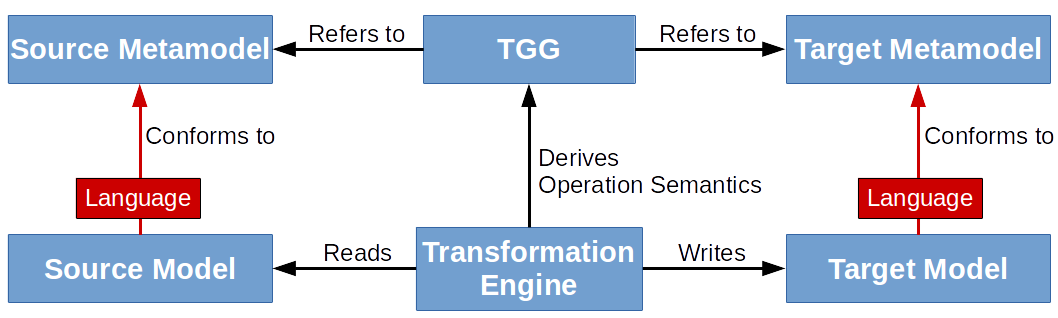
\includegraphics[width=25em]{transformation_scheme}
    \end{center}
    \label{fig:transformation_scheme}
    \legend{Source: Adapted from \citet[p. 623]{czarnecki2006feature}}
\end{figure}

\end{description}
 
\section{Related Work}
%TODO: us?
A work similar to the one of this thesis, which builds a network of meta-models of the Java technogical space, by describing them and their intrinsic relations is not known by us. In this sense the results of this thesis is novel and contributive. Nevertheless some endeavors have been made in order to code relations between some meta-models and mainly to develop theoretical results and synchronization methods. \citeauthor{heidenreich2010closing} present in \citeyearpar{heidenreich2009jamopp} and \citeyearpar{heidenreich2010closing} a Java meta-model using \emph{Ecore}, what influenced considerably the development of our work, although it has not been used by us because of its size and unnecessary comprehensibility for our needs. \citet{greenyer2008tggs} comes up with a transformation between \emph{UML activity diagrams} and \emph{CSP diagrams} using \emph{TGG}. \citet{foss2011uml} defined the translation between \emph{UML} and \emph{Simulink} using graph grammars. \citet{blouin2014synchronization} reports about the synchronization between some specific meta-models of the automotive standards and influences our work, by using the same modeling language and synchronization method as us, namely \emph{EMF} \citep{steinberg2008emf} and \emph{MoTE} \citep{giese2010toward}. Finally \citet{giese2010model} introduce their approach to the synchronization of two automotive industry meta-models, lightening in the paper the \emph{MoTE} tool and its algorithm for synchronization.

We judge that the \emph{MoTE} tool is the most adequate option for our needs, once literature about it is widely available (see also \citep{giese2009efficient} and \citep{hildebrandt2012mdelab}). Nevertheless there are other attempts to build a model synchronization tool, like the \emph{ATL Eclipse Plug-in} \citep{jouault2008atl}, which uses the \emph{Atlas Transformation Language} to code the relations between models; the Medini QVT \footnote{http://projects.ikv.de/qvt}, which claims to implement the \emph{Query/View/Transformation Language} to code the relations; and the FUJABA \citep{nickel2000fujaba}, in which relations are coded using \emph{Triple Graph Grammars}. \citet{hildebrandt2013survey} also publicized a survey on synchronization tools based on TGG. Other publications aim to solve specific problems, like the ones in \citet{hermann2011correctness}, \citet{xiong2007towards}, \citet{giese2006incremental}, \citet{ivkovic2004tracing}, or \citet{song2011instant}, where advanced algorithms for bidirectional synchronization have been proposed.

A research road-map for model synchronization found in \citet{france2007model} gives an overview on the realm, and together with \citet{mattsson2009linking} show an interesting point of view about the challenges. \citet{seidewitz2003models} writes an interesting reflection  about what models mean and how to interpret them and in \citet{mens2006taxonomy} a taxonomy for model transformation is proposed, what helps to carry more precise analysis. In \citet{czarnecki2006feature} a survey was driven and a framework for classification of model transformation approaches was presented. In \citeauthor{diskin2014towards} \citeyearpar{diskin2014towards} and \citeyearpar{diskin2016three} a taxonomy for a network of models is presented and in \citet{diskin2011model} a theoretical algebraic basis is proposed.

Additionally, one can judge by the date of publication of these works, that the topic of model synchronization is extremely active and is actually the edge of current academic research, what motivates even more the development of this thesis.

\chapter{Meta-model Relations in the Java Technological Space}
\section{Meta-models}
%TODO: Quote emf
%TODO: emf-ecore = Language?
%TODO: Site Eclipse
The language(?) used to write these meta-models is the EMF Ecore [QUOTE EMF] and the Eclipse IDE \footnote{SITE} is used as tool to such work.
%TODO: img 45 p563
Possibly, simplifications on the meta-models shall be done, so that they fit the necessities of our scope, and can be made using the \emph{EMF} standard \cite{steinberg2008emf}.
\section{Relations}

\chapter{Synchronization Between Some Models in the Java Technological Space}
%TODO: assumptions: no paralel changes(one change at a time); direction given ...

\chapter{Conclusion and Discussion}

%TODO: Adjust to UFRGS style? see iiufrgs
\bibliographystyle{plainnat}
\bibliography{biblio}

\end{document}
